%! Author = Ian
%! Date = 11/28/2023

% Preamble
\documentclass{article}

% Packages
\usepackage{amsmath}
\usepackage{fancyhdr}
\usepackage[top=2cm, left=2cm, right=2cm, bottom=2cm]{geometry}
\usepackage{multicol}
\usepackage{amsfonts}
\usepackage{gensymb}
\usepackage{graphics}
\usepackage{graphicx}

\setlength{\columnsep}{0.5cm}

\author{Ian Chen}
\date{\today}

% Header
\fancyhf{}
\fancyhead[L]{Ian Chen}
\fancyhead[C]{CS376 Notes}
\fancyhead[R]{ic8683}
\pagestyle{fancy}

% Document
\begin{document}
    \begin{multicols*}{2}
        \subsubsection*{Structure from Motion}
        Estimates intrinsic and extrinsic parameters, which characterize the search space\newline
        \textit{Pinhole Camera}: Dominant image formation model in computer vision\newline
        \textit{Homogenous Coordinates}: (x, y) $\leftrightarrow$ ($\lambda$x, $\lambda$y, $\lambda$)\newline
        \textit{Intrinsic Parameters}: K-Matrix, optical center and focal length\newline
        \textit{Extrinsic Parameters}: [R$\mid$t], location of the camera in the 3-D scene\newline
        \textit{Projection Matrix}: $\Pi$ = K[R$\mid$t]\newline
        \textit{Fundamental Matrix}: Uses in/extrinsic, pixel to epipolar line\newline
        \textit{Essential Matrix}: Uses intrinsic, TR, 5$\degree$ of freedom, 8-point
        algorithm, rank=2\newline
        \textit{Epipolar Geometry}: Two views
        \subsubsection*{Camera Calibration}
        X = [X, Y, Z, W]$^T$, W = 1\newline
        \textit{Image Plane}: x = [x y 1]$^T$\newline
        \textit{Camera Extrinsic}: g = (R, T)\newline
        \textit{Perspective Projection}: $\lambda$x = [R, T]X\newline
        \textit{Pixel Coordinates}: x' = Kx\newline
        \textit{Projection Matrix}: $\lambda$x' = $\Pi$X = [KR, KT]X\newline
        \textit{Rig}: Known coordinates
        \subsubsection*{Stereo Matching}
        Recovers depth\newline
        \textit{Binocular Stereo}: Find corresponding epipolar line, if same height, then
        scan lines\newline
        \textit{Non-Local Constraint}: Point in one image corresponds to one point in other image\newline
        \textit{Ordering}: Corresponding points should be in same order\newline
        \textit{Window Search}: More noise in depth map\newline
        \textit{Markov Random Field}: Graphical model of joint PDF\newline
        \textit{Graph Cut}: Less noise, minimize energy
        \subsubsection*{Image Classification}
        \textit{Cross-Validation}: Split training set into n-folds, [0, n-1] for training, [n] for
        testing
        \subsubsection*{KNN}
        Influenced by size of training set, works well for large training sets\newline
        \textit{Hyperparameters}: K and Norm(L1 better, reduces background noise)\newline
        \textit{Pros}: Simple\newline
        \textit{Cons}: Expensive(Use PCA), Norm choice\newline
        \textit{Curse of Dimensionality}: Overfitting
        \subsubsection*{Linear Classifier}
        Foundation in neural networks\newline
        \textit{Score Function}: Map data to class scores\newline
        \textit{Loss Function} Quantifies prediction/ground truth disparity
        \subsubsection*{SVM}
        SVM: Hinge loss | Softmax: Cross-entropy loss\newline
        More efficient and works better than KNN with modest training datasets\newline
        \textit{Multi-Class Loss} Data loss + Regularization loss
        \subsubsection*{Softmax Classifier}
        Provides probabilities for each class\newline
        \textit{Cross-Entropy Loss}: Maximize cross-entropy
        \subsubsection*{AdaBoost}
        Ensemble method, combine weak(base) learners to form strong learner, robust to
        overfitting, not identical to SVM
        \subsubsection*{Viola-Jones Face Detector}
        Uses AdaBoost\newline
        \textit{Haar-like Features}: +/- Rectangles\newline
        \textit{Integral Image}: II$_{ij}$ = $\sum$i$_{x\leq i;y \leq j}$ \newline
        \textit{Classifier Cascade}: Each successive strong classifier uses more features, lower
        threshold to reduce false negative(increase false positive), Every classifier must be
        positive to be classified as positive
        \subsubsection*{Neural Network}
        Layers of neurons, each neuron is a linear classifier, each layer is a non-linear
        transformation\newline
        \textit{Score Function}: Employs non-linear activation function\newline
        \textit{R-CNN}: Pre-trained, fine-tuned on PASCAL VOC
        \subsubsection*{Pooling Layer}
        Downsamples spatial dimensions, reduces computation\newline
        \textit{Max Pooling}: Take max of each window to downsample
        \subsubsection*{Fully-Connected Layer}:
        \textit{Neurons} Connected to every neuron of next layer
        \subsubsection*{Convolutional Layer}
        Colloquially uses cross-correlation, uses CONV/FC/POOL layers\newline
        \textit{Output Size(Image$_{N\times N}$, Filter$_{F \times F}$)}: (N - F)/(stride + 1)\newline
        \textit{Stride}: Jump of filter over image\newline
        \textit{Padding}: To make output same size\newline
        \textit{Hyperparameters}: \# filters, filter size, stride, padding
        \subsubsection*{Gradient Descent}
        \textit{Numerical}: Slow, Approximate, Easy to Write\newline
        \textit{Analytic}: Fast, Exact, Error Prone
        \subsubsection*{Backpropagation}
        \textit{Forward/Backward API}: Forward- Compute operations, save immediates for gradient
        computation, Backward- Apple chain rule to compute gradient of loss function
        \subsubsection*{Object Detection}
        \textit{Window-Based}: Viola-Jones, Strengths- Simple detection protocol, good feature
        choices critical, past successes for certain classes, Flaws- High computational
        complexity, need low false positive rates, not all objects box shaped, assumes fixed
        viewpoint
        \subsubsection*{Conv-DeConv}
        Alternate convolve and max pooling, then deconvolving and unpooling
        \subsubsection*{Object Proposals}
        \textit{Proposals}: Object-like regions\newline
        \textit{Person Detection}: HoG and linear SVM\newline
        \textit{Dalal-Triggs Method}: Sliding Window, HoG, + linear SVM\newline
        \textit{Deformable Part Model}: Star Model- Coarse Root Filter + Higher resolution part
        filters\newline
        \textit{Object Hypothesis}: Level+Position of the i-th filter
        \subsubsection*{Active Contour}
        Used in segmentation\newline
        \textit{Snakes}: Match curve by minimizing energy
        \subsubsection*{Decision Tree}
        Testing attribute should split training samples into subsets that are as pure as possible\newline
        \textit{Leaves}: Decisions\newline
        \textit{Information}: Reduction in uncertainty\newline
        \textit{Entropy}: Expected amount of information\newline
        \textit{Information Gain}: Information before split - after\newline
        \textit{Bagging}: Reduce variance, committee of trees, samples with replacement\newline
        \textit{Random Forest Classifier}: ex. Microsoft Kinect, efficient, distributed,
        variable importance, easy to update algorithm, cons: interpretability\newline
        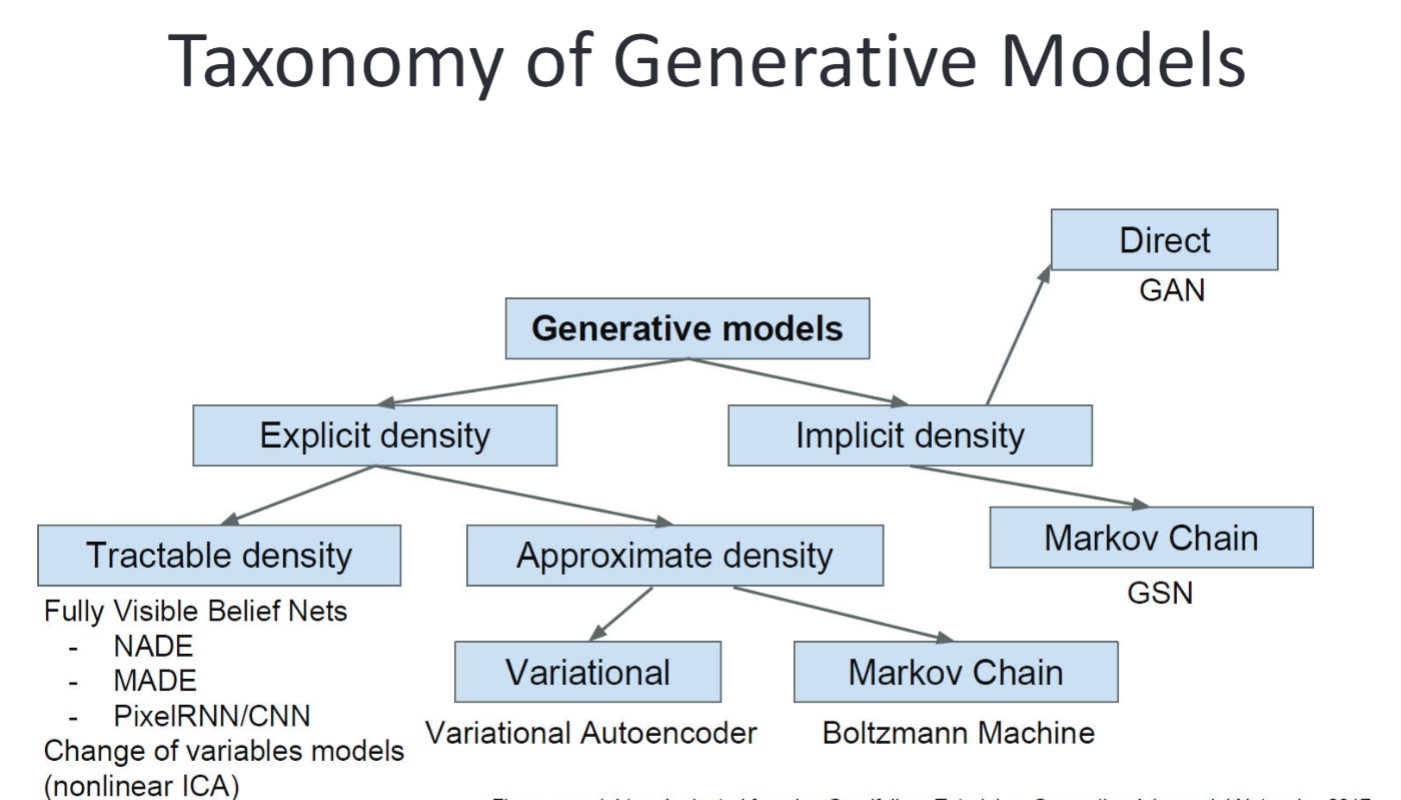
\includegraphics[width=0.5\textwidth]{generative_models}
        \subsubsection*{Generative Models}
        Synthesize images, generate training data, serve sub-modules\newline
        \textit{Generative Adversarial Networks}: Sample from simple distribution, learn
        transformation to training distribution\newline
        \textit{Generative Network}: Try to fool discriminator by generating real-looking images\newline
        \textit{Discriminator Network}: Try to distinguish real/fake images\newline
        \textit{Variational Autoencoder}: Autoencoder- Reconstruct data, Pros- Principled
        approach to generative models, allows inference of q(z$\mid$x), can be useful feature
        representation in other tasks, Cons- Maximizes lower bound of likelihood
        \subsubsection*{U-Net}
        Designed for biomedical image segmentation, featuring a U-shaped structure with
        contracting and expanding paths to capture context and spatial information effectively.
        \subsubsection*{ResNet}
        Helps with vanishing gradients with residual blocks, used in image classification
        \subsubsection*{Semantic Segmentation}
        \textit{Applications}: TextonBoost, Conv-Deconv, Dilated-Conv\newline
        \textit{Markov Random Field}: Smooth\newline
        \textit{Sliding Window}: Approach 1, can use early stop using more efficient classifiers\newline
        \textit{Fully Convolutional}: Approach 2
        \subsubsection*{Instance Segmentation}
        \textit{FCN Methods}: Divide results from semantic segmentation into individual instances\newline
        \textit{RCNN Methods}: Use segmentation level proposals then train classifier to classify
        proposals
    \end{multicols*}
\end{document}